\documentclass[tikz,border=10pt]{standalone}
\usepackage{tikz}
\usepackage{pgfplots}
\pgfplotsset{compat=1.16}

\begin{document}

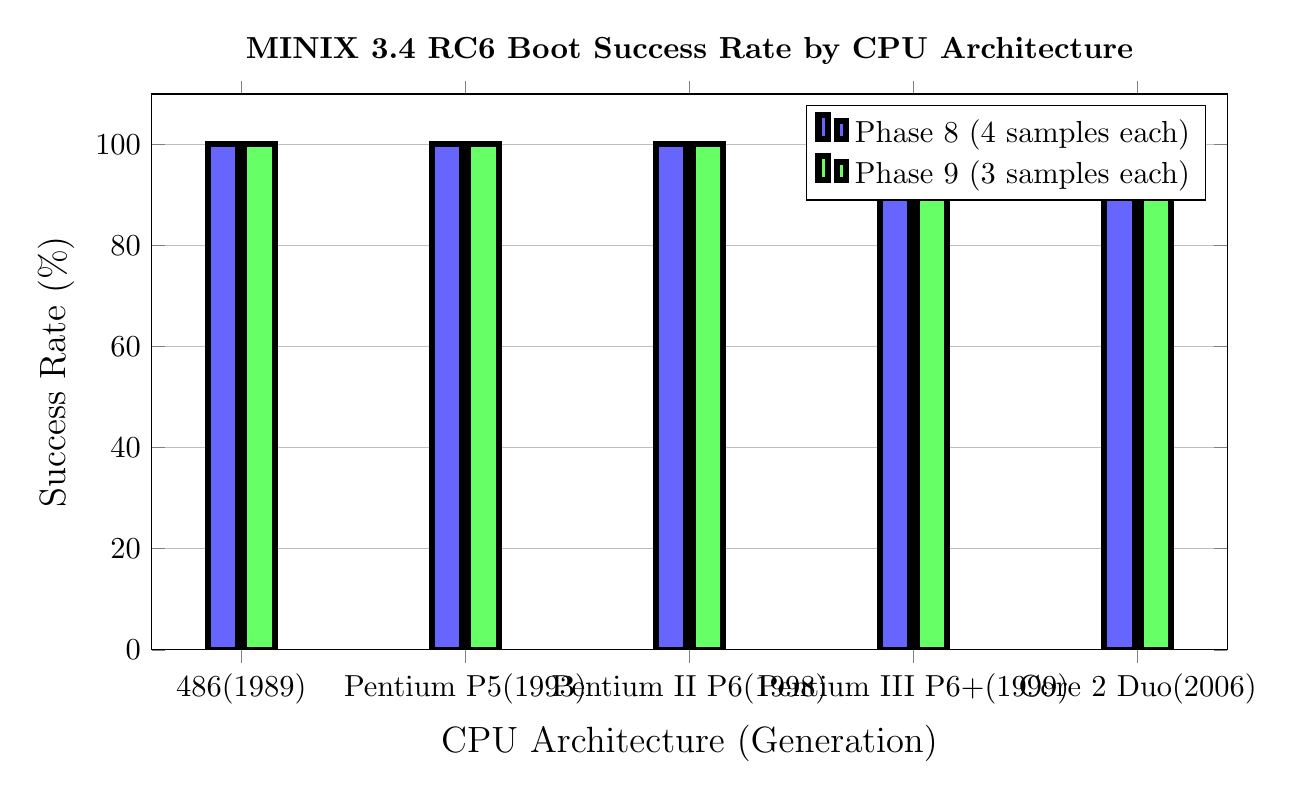
\begin{tikzpicture}[scale=1.1]
  \begin{axis}[
    title={MINIX 3.4 RC6 Boot Success Rate by CPU Architecture},
    xlabel={CPU Architecture (Generation)},
    ylabel={Success Rate (\%)},
    ybar,
    width=14cm,
    height=8cm,
    ymin=0, ymax=110,
    ymajorgrids=true,
    xtick={1,2,3,4,5},
    xticklabels={
      486\\(1989),
      Pentium P5\\(1993),
      Pentium II P6\\(1998),
      Pentium III P6+\\(1999),
      Core 2 Duo\\(2006)
    },
    ylabel style={font=\large},
    xlabel style={font=\large},
    title style={font=\Large, font=\bfseries},
    ]

    % Phase 8 results (20/20 on supported CPUs)
    \addplot[fill=blue!60, draw=black, line width=2pt]
      coordinates {
        (1, 100)
        (2, 100)
        (3, 100)
        (4, 100)
        (5, 100)
      };
    \addlegendentry{Phase 8 (4 samples each)};

    % Phase 9 results (15/15 total, 100\% on all)
    \addplot[fill=green!60, draw=black, line width=2pt]
      coordinates {
        (1, 100)
        (2, 100)
        (3, 100)
        (4, 100)
        (5, 100)
      };
    \addlegendentry{Phase 9 (3 samples each)};

  \end{axis}
\end{tikzpicture}

\end{document}